\documentclass[french, a4paper, 12pt, titlepage]{article}
%% Peut remplacer "article" par "scrartcl" %%

\usepackage{a4wide}
%\usepackage[top=2cm, bottom=2cm, left=2cm, right=2cm]{geometry}
\raggedbottom%  Prevents vertical white space on pages that cannot be filled properly

\usepackage{microtype}
\usepackage{hyperref}
\hypersetup{%
	colorlinks=true,       	% false: boxed links; true: colored links
	linkcolor=black,          	% color of internal links
	urlcolor=blue,           	% color of external links
	citecolor=grey
}

\usepackage[T1]{fontenc}
%\usepackage{fourier}
%\usepackage{utopia}
%\usepackage{palatino}

\usepackage{lmodern}
%% ajouter fonte petite capitale grasse à lmodern avec celle de computer modern %%
\rmfamily
\DeclareFontShape{T1}{lmr}{b}{sc}{<->ssub*cmr/bx/sc}{}
\DeclareFontShape{T1}{lmr}{bx}{sc}{<->ssub*cmr/bx/sc}{}
%% /ajout %%
\usepackage{wrapfig}

%\usepackage[a4paper]{geometry} % marges plus petites que a4paper standard
%\usepackage{algorithm} % algorithmique
%\usepackage{algorithmic}
\usepackage{url}
\usepackage[usenames, dvipsnames]{color} % couleurs (nombre de base étendu)
\usepackage{graphicx} % insérer images
\usepackage[utf8]{inputenc}
\usepackage[french]{babel}
\usepackage{listings}% insérer code source
\lstloadlanguages{sh,bash,awk,make}
\usepackage{amsmath}
\usepackage{amsfonts}
\usepackage{amssymb}
\usepackage{amsthm}
\usepackage{multicol}
\definecolor{grey}{rgb}{0.96,0.96,0.96}
\definecolor{grey2}{rgb}{0.3,0.3,0.3}

%% Define listings params %%
\lstset{%
%	numbers=left,
	language=bash,
	tabsize=4,
	frame=single, % cadre autour du code
	breaklines=true, % autorise couper ligne trop longue
	basicstyle=\small\ttfamily,
	numberstyle=\scriptsize\ttfamily,
	backgroundcolor=\color{grey},
	showstringspaces=false,
	keywordstyle=\color{OliveGreen},
	stringstyle=\color{BrickRed},
	commentstyle=\color{grey2}\it,
	stepnumber=1 % numérote toute les x lignes
}
% listing utf8 fr %
\lstset{%
	inputencoding=utf8,
	extendedchars=true,
	literate=
		{é}{{\'{e}}}1
		{è}{{\`{e}}}1
		{ê}{{\^{e}}}1
		{ë}{{\"{e}}}1
		{û}{{\^{u}}}1
		{ù}{{\`{u}}}1
		{â}{{\^{a}}}1
		{à}{{\`{a}}}1
		{î}{{\^{\i}}}1
		{ç}{{\c{c}}}1
		{Ç}{{\c{C}}}1
		{É}{{\'{E}}}1
		{Ê}{{\^{E}}}1
		{À}{{\`{A}}}1
		{Â}{{\^{A}}}1
		{Î}{{\^{I}}}1
}
%% /Define listings params %%

%% Francisation des algorithmes
%\renewcommand{\algorithmicrequire} {\textbf{\textsc{Entrées:}}}
%\renewcommand{\algorithmicensure}  {\textbf{\textsc{Sorties:}}}
%\renewcommand{\algorithmicwhile}   {\textbf{tant que}}
%\renewcommand{\algorithmicdo}      {\textbf{faire}}
%\renewcommand{\algorithmicendwhile}{\textbf{fin tant que}}
%\renewcommand{\algorithmicend}     {\textbf{fin}}
%\renewcommand{\algorithmicif}      {\textbf{si}}
%\renewcommand{\algorithmicendif}   {\textbf{fin si}}
%\renewcommand{\algorithmicelse}    {\textbf{sinon}}
%\renewcommand{\algorithmicthen}    {\textbf{alors}}
%\renewcommand{\algorithmicfor}     {\textbf{pour}}
%\renewcommand{\algorithmicforall}  {\textbf{pour tout}}
%\renewcommand{\algorithmicdo}      {\textbf{faire}}
%\renewcommand{\algorithmicendfor}  {\textbf{fin pour}}
%\renewcommand{\algorithmicloop}    {\textbf{boucler}}
%\renewcommand{\algorithmicendloop} {\textbf{fin boucle}}
%\renewcommand{\algorithmicrepeat}  {\textbf{répéter}}
%\renewcommand{\algorithmicuntil}   {\textbf{jusqu'à}}
%\renewcommand{\algorithmiccomment} {\STATE //}
%\newcommand{\BEGIN}{\STATE \fbox{Début}}
%\newcommand{\END}{\STATE \fbox{Fin}}
%\floatname{algorithm}{Algorithme}
%% /francisation des algorithmes

\renewcommand{\qedsymbol}{}

\newcommand{\petit}[1]{%
	\medskip \noindent
	\begin{small}
	#1)
	\end{small}
}

\begin{document}
\title{Introduction à Git}
%\author{
\includegraphics{clubnix}}
\author{
\includegraphics{clubnix}}
\date{\url{https://clubnix.fr}}

\maketitle
%% Laisse page blanche pour verso page de garde %%

\vfill
\pagebreak

%\tableofcontents
\newpage
\strut\thispagestyle{empty}
\vfill
\pagebreak
\tableofcontents
\strut\thispagestyle{empty}
%\setcounter{page}{0}
\newpage
\setcounter{page}{1}

\part{Introduction}

\section{Les gestionnaires de versions}

\paragraph{} Un gestionnaire de version est un outil permettant de maintenir plusieurs versions, c'est-à-dire qu'il est capable d'enregistrer les différents états d'un ou de plusieurs fichiers au cours du temps et de naviguer facilement entres ses états.

\paragraph{}Il en existe plusieurs, les plus connus étant \emph{mercurial}, \emph{SVN} et \emph{Git}.  Nous nous intéresserons uniquement à ce dernier qui est notamment utilisé pour la réalisation de Linux.

\section{Git, GitLab, GitHub: fonctionnement et différences}

\paragraph{}Vous qui lisez ce tutoriel, vous avez sûrement déjà entendu parler de GitHub et/ou GitLab alors que dans ce poly, nous allons uniquement vous détailler git.

Pourquoi ? Tout simplement parce-que git est en fait le coeur du fonctionnement de GitHub et GitLab \emph{(ce n'est pas rien qu'ils s'appelent tous les deux Gitquelque-chose...)}. En effet, tout le fonctionnement détaillé dans ce poly est le même pour ces trois outils, alors quelle sont les différences ?

\paragraph{}Pour faire court git a un fonctionnement qui ne nécessite aucune centralisation, ou autrement dit aucun serveur ou tout le monde rassemble son travail. Mais la plupart du temps, les équipes préférent avoir un dépôt cental où l'on peut retrouver le projet avec les dernières modifications. Et c'est avec cet esprit que GitHub est né. En plus de cela, sans compte payant, les projets qui utilisent GitHub, sont entièrement accessible par tous (Open Source), par contre, pour avoir un dépôt privé, il faut avoir un compte payant.

Mais dans ce cas là, comment peut faire une petite équipe de développeurs ou
même une très grosse entreprise qui désire utiliser Git avec un outil clés en
main mais avec des dépôts privés ET sans payer ? C'est là où est arrivé GitLab.
Ce dernier outil propose un outil avec autant (ou presque ou plus selon les
années...) que GitHub mais de façon entièrement Open Source. Ainsi, n'importe
qui peut installer un serveur GitLab pour lui ou son équipe et en faire ce
qu'il veut (public et/ ou privé). GitLab possède aussi des fonctionnalités
payantes non Open-Source.

\paragraph{}Dernier \emph{détail}, le logiciel Git est Open Source (c'est grâce
à cela que les deux autres outils peuvent se baser dessus) et n'appartient pas
à une entreprise, contrairement à GitLab, et GitHub qui appartient à Microsoft
depuis 2018.

%
% \paragraph{} Git a la particularité, contrairement à d'autres gestionnaires de version d'être décentralisé, c'est à dire qu'il n'a pas besoin d'un serveur pour fonctionner.  Cependant pour des raisons de simplicité il est souvent utilisé de cette manière.
% %TODO ref plus loin
%
% \paragraph{} Chaque personne possède un dépôt privé, et un dépôt public.  Le dépôt privé sert à faire du développement local, et le public sert à envoyer des versions du code source afin que d'autres personnes puissent les télécharger. En donnant à tout un groupe d'utilisateurs le même dépôt public, le système devient alors centralisé. De cette manière,tout le monde peut connaître la progression de chacun des utilisateurs dans le projet.
%
% Enfin, les gestionnaires de versions apportent une sécurité supplémentaire dans le cas où le serveur qui permettait aux utilisateurs de collaborer s'arrêterait. En effet, chaque collaborateur serait alors capable de le restaurer en recopiant leur dépôt sur le serveur centralisé.

\newpage
\part{Installation}
\paragraph{}L'installation de Git diffère en fonction de votre système d'exploitation:
\section{Linux}
\paragraph{} Pour installer Git sur un système Linux il suffit d'exécuter la commande suivante:

\begin{lstlisting}
$ sudo apt-get install git
\end{lstlisting}

\paragraph{} A savoir que Git est installé par défaut sur certains systèmes
Linux. Si vous voulez aussi une interface graphique, plutôt que d'utiliser git
exclusivement en ligne de commande vous pouvez aussi installer "gitk" en
exécutant:

\begin{lstlisting}
$ sudo apt-get install gitk
\end{lstlisting}

\section{Windows}
\paragraph{}Pour les systèmes Windaub, il faut installer \emph{msysgit} qui installera un terminal Unix permettant d'utiliser les commandes Linux de Git (et donc de suivre la suite du tuto) ainsi que les paquets Git essentiels à son bon fonctionnement, pour installer msysgit reportez-vous au tutoriel fourni sur \url{http://msysgit.github.io}

\section{MacOS}
\paragraph{}Il y a plusieurs façons d’installer Git sous Mac OS X. Le plus simple est de se baser sur cet installeur pour Mac OS X:

\url{https://code.google.com/archive/p/git-osx-installer/}.

\paragraph{} MacOS utilisant un terminal Linux nous pourrons utiliser les
commandes données dans ce tuto sous MacOS.

\newpage
\part{Configuration de Git}
\paragraph{}Avant de commencer à utiliser Git il vous faudra créer une configuration basique de Git, pour cela il vous faudra seulement exécuter quelques commandes dans un terminal Linux afin de configurer \emph{votre} Git en ajoutant votre nom et votre mail:
\begin{lstlisting}
$ git config --global user.name "VotrePseudo"
$ git config --global user.email moi@email.com
\end{lstlisting}

\newpage
\part{Création de dépôt local}

\section{Clonage d'un dépôt distant}

\paragraph{} La manière la plus fréquente de créer un dépôt
(\emph{repository}) Git est le "clonage", c'est-à-dire la copie entière d'un projet géré avec Git. Si l'on prend par exemple le projet de ce cours même qui est stocké sur \href{https://github.com}{GitHub} à l'adresse
\url{https://github.com/ClubNix/tuto-git}, il suffit de taper la commande suivante pour copier le projet entier dans le dossier courant~:

\begin{lstlisting}
$ git clone https://github.com/ClubNix/tuto-git.git
\end{lstlisting}
\paragraph{}Il est aussi possible de manière facultative de spécifier dans quel dépôt le clonage va se faire:
\begin{lstlisting}
$ git clone https://github.com/ClubNix/tuto-git.git dossier
\end{lstlisting}

\paragraph{} L'URL de clonage vous est normalement fournie par le service que
vous utilisez pour héberger votre code (GitHub, GitLab ou autre). Attention: il
est possible que l'URL de clonage ne soit pas la même que l'URL utilisée pour
voire votre projet sur votre navigateur internet.

\section{Création d'un dépôt vide}

\paragraph{} Il est bien sûr possible avec Git de créer un dépôt vide. Pour cela, il suffit de faire la commande suivante dans le dossier créé pour stocker le dépôt Git:

\begin{lstlisting}
$ git init
\end{lstlisting}

\paragraph{} Cela va tout simplement ajouter les fichiers propres à Git dans le répertoire courant ainsi qu'initialiser la gestion de version.

\paragraph{} Notez qu'il est souvent plus simple de créer un dépôt vide
directement sur GitHub ou GitLab, puis de le cloner, car Git sera à ce moment
là assez malin pour "lier" votre dépôt local à celui distant.

\newpage
\part{Exemple d'un workflow avec Git}
\paragraph{} Avec Git, un workflow courant, est constitué de 4 étapes : la modification, la validation, le commit et l'envoi. Nous allons voir chacune des étapes dans cette partie.
\section{Modification}
\paragraph{}La modification est tout simplement le moment pendant lequel les fichiers (de code, etc\dots) sont modifiés. C'est la partie qui semble la plus simple dans la gestion de version. Cependant, afin d'exploiter la gestion de version à son plein potentiel, certaines règles doivent être respectées.
\paragraph{}Premièrement, Git analyse les différents changement en faisant des "diff", qui consistent à regarder le différences entre un même fichier à des versions antérieures. Ainsi, afin de clarifier un peu le tout, il est conseillé de préférer du texte sur plusieurs lignes que du texte sur une seule ligne.

Ensuite, afin de pouvoir mieux gérer son dépôt mais aussi de mieux gérer la stabilité et la fonctionnalité du projet, il est aussi conseillé de maximiser le nombre de versions et d'en valider une aussitôt que le projet ``fonctionne''. Cela facilitera grandement la détection et la résolution d'erreurs mais aussi le travail avec les branches que l'on verra plus tard.


\newpage
\part{Quelle procédure suivre pour enregistrer vos fichiers}
\paragraph{}La procédure pour utiliser Git va être la suivante:
\begin{itemize}
\item On ajoute tous les fichiers qui seront à enregistrer sur le dépôt distant grâce à la commande "add"
\item On "commit" tous les changements de fichier sur notre dépôt local, cela aura pour effet de les enregistrer en créant une version locale du projet en attente de l'envoi sur le dépôt distant,
\item On "push" tout notre commit sur le dépôt distant afin d'enregistrer nos modifications sur celui-ci, la version locale précédemment crée est envoyée et devient similaire à la version distante.
\end{itemize}

\paragraph{}Nous verrons en détail toutes ces commandes dans la suite de ce tuto, il est à noter que certaines commandes de vérifications que nous verrons peuvent être utilisées entre chaque étape afin de vérifier les fichiers que vous envoyez ou qu'il n'y a tout simplement pas d'erreur.

\newpage
\part{Les commandes Git de base}
\paragraph{}Arrivé à ce stade, vous savez créer un nouveau dépôt ou en cloner un existant afin de travailler dessus, nous allons donc maintenant voir les commandes de base pour effectuer des "sauvegardes" de votre dossier Git:

\section{Obtenir de l'aide}

\paragraph{} Si vous voulez des informations sur une commande particulière,
vous pouvez utiliser la commande "git help". Par exemple, si vous voulez de
l'aide sur la commande "git status" (que nous allons voir juste après), vous
pouvez exécuter dans un terminal:

\begin{lstlisting}
$ git help status
\end{lstlisting}

\paragraph{} Git est très bien documenté, alors n'hésitez pas.

\section{Modifier le code et effectuer des commits}
\subsection{git status}
\paragraph{}Lorsque vous modifiez les fichiers contenus dans votre dépôt Git vous devez les envoyer sur le serveur afin de les sauvegarder pour l'ensemble des développeurs, pour cela vous pouvez utiliser la commande suivante afin de voir les fichiers qui ont été modifiés mais dont les modifications ne sont pas enregistrées sur le dépôt:
\begin{lstlisting}
$ git status
\end{lstlisting}

\paragraph{}Pour aller plus loin nous pouvons même voir en détail les modifications non enregistrées grâce à la commande suivante:
\begin{lstlisting}
$ git diff
\end{lstlisting}

\subsection{git commit}
\paragraph{}Maintenant que vous savez quelle modification sont a enregistrer nous pouvons passer au commit de ces changements. Pour cela plusieurs methodes sont possible:

\paragraph{}La première va consister à ajouter les fichiers qui ont été modifiés dans le tas des fichiers à commit:
\begin{lstlisting}
$ git add nomfichier1 nomfichier2
\end{lstlisting}
vous pouvez aussi ajouter tous les fichiers en même temps en utilisant :
\begin{lstlisting}
$ git add .
\end{lstlisting}

\paragraph{}Puis de commit ces fichiers grâce à la commande:
\begin{lstlisting}
$ git commit
\end{lstlisting}
\paragraph{}Cette commande va tout d'abord vous demander d'écrire un message pour votre commit. Nous ne nous étendrons pas dessus ici, mais, un message de commit doit être clair et concis. Quelqu'un qui n'était pas avec vous quand vous avez fait un certain commit doit pouvoir comprendre le but et l'intérêt du commit uniquement grâce à son message.

Par défaut git commit ouvrira un éditeur de texte intégré au terminal pour que vous le tapiez. Pour éviter cela vous pouvez passer le message en paramètre de la commande commit ainsi :
\begin{lstlisting}
$ git commit -m "Votre message clair et concis."
\end{lstlisting}

Le commit aura pour effet de créer une sauvegarde/version du dépôt local sur votre ordinateur, sauvegarde que vous pourrez envoyer sur le dépôt distant par la suite.

NB: Après un \emph{git add ...} si vous faites un \emph{git status} vous verrez les fichiers ajoutés apparaître en vert.

\paragraph{}La deuxième méthode consiste à "commiter" tous les fichiers qui étaient listés dans \emph{git status} dans les colonnes "Changes to be committed" et "Changed but not updated" (qu’ils soient en vert ou en rouge) grâce à la commande :
\begin{lstlisting}
$ git commit -a
\end{lstlisting}
Cette dernière ligne est donc équivalente à la suite suivante :
\begin{lstlisting}
$ git add .
$ git commit
\end{lstlisting}

\paragraph{}La troisième solution va consister à indiquer à Git quels fichiers doivent être commit :
\begin{lstlisting}
$ git commit nomFichier1 nomFichier2
\end{lstlisting}

\subsection{Annuler un commit}
\paragraph{}Dans le cas où vous auriez commité des erreurs il est encore possible d'annuler le dernier commit effectué.
\paragraph{}Pour cela nous allons commencer par vérifier les logs:
\begin{lstlisting}
$ git log
\end{lstlisting}

\paragraph{}Vous devriez normalement voir tous les derniers commit effectués.
Chaque commit est numéroté grâce à un long numéro hexadécimal comme
\textit{12328a1bc\ldots} Cela permet de les identifiers.

\paragraph{}Pour aller plus loin vous pouvez voir les lignes modifiées par le commit en utilisant la commande suivante :
\begin{lstlisting}
$ git log -p
\end{lstlisting}
\paragraph{}Vous pouvez aussi avoir un résumé plus court des commits avec :
\begin{lstlisting}
$ git log --stat
\end{lstlisting}

\paragraph{}Dans le cas où vous auriez fait une faute dans le message de votre dernier commit il existe une commande permettant d'ouvrir un éditeur de texte pour le modifier :
\begin{lstlisting}
$ git commit --amend
\end{lstlisting}
\paragraph{}Mais attention, il est en effet impossible de modifier le message d’un commit lorsque celui-ci a été transmis à d’autres personnes. Elle s'utilise daonc avant le push.
\paragraph{}Pour annuler votre dernier commit vous pouvez utiliser la commande suivante:
\begin{lstlisting}
$ git reset HEAD^
\end{lstlisting}
\paragraph{}Cela annule le dernier commit et revient à l’avant-dernier.
\paragraph{}Pour indiquer à quel commit on souhaite revenir, il existe plusieurs notations :
\begin{lstlisting}
-HEAD : dernier commit ;
-HEAD^ : avant-dernier commit ;
-HEAD^^ : avant-avant-dernier commit ;
-HEAD~2 : avant-avant-dernier commit (notation équivalente) ;
-d6d98923868578a7f38dea79833b56d0326fcba1 : indique un numéro de commit précis.
\end{lstlisting}
\paragraph{}Seul le commit est retiré de Git ; vos fichiers, eux, restent modifiés. Vous pouvez alors à nouveau changer vos fichiers si besoin et refaire un commit.
\paragraph{}Vous pouvez aussi annuler un commit et \emph{toutes} les modifications qu'il implique grâce à la commande:
\begin{lstlisting}
$ git reset --hard HEAD^
\end{lstlisting}

\subsection{Restaurer un fichier à son état antérieur avant le commit}
\paragraph{}Si vous avez modifié plusieurs fichiers mais que vous n’avez pas encore envoyé le commit et que vous voulez restaurer un fichier tel qu’il était au dernier commit, utilisez:
\begin{lstlisting}
$ git checkout nomfichier
\end{lstlisting}
\paragraph{}Il est possible de retirer un fichier qui avait été ajouté pour être "commité" en procédant comme suit:
\begin{lstlisting}
$ git reset HEAD -- fichier_a_supprimer
\end{lstlisting}

Ces deux dernières commandes peuvent se retrouver dans le commentaires affichés par la commande git status.

\section{Partager votre travail et télécharger les nouveautés}
\paragraph{}Sous Git, vous travaillez sur un dépôt local, mais tous les fichiers du projet sont aussi contenus sur un dépôt distant dans lequel tous les contribueurs peuvent faire des modifications. Il sera donc nécessaire de savoir télécharger les nouveautés apportées par d'autres mais aussi de savoir envoyer vos nouveautés sur le dépôt distant.
\subsection{Télécharger les nouveautés}
\paragraph{}Pour télécharger les nouveautés du dépôt il vous suffit d'utiliser la commande suivante:
\begin{lstlisting}
$ git pull
\end{lstlisting}
\paragraph{}Deux cas sont possibles :
\begin{itemize}
\item Soit vous n’avez effectuée aucune modification depuis le dernier pull, dans ce cas la mise à jour est simple (on parle de mise à jour fast-forward) ;
\item Soit vous avez fait des commits en même temps que d’autres personnes. Les changements qu’ils ont effectués sont alors fusionnés aux vôtres automatiquement.
\end{itemize}

\paragraph{}Si deux personnes modifient en même temps deux endroits distincts d’un même fichier, les changements sont intelligemment fusionnés par Git.

Parfois, mais cela arrive normalement rarement, deux personnes modifient la
même zone de code en même temps. Dans ce cas, Git dit qu’il y a un conflit car
il ne peut décider quelle modification doit être conservée ; il vous indique
alors le nom des fichiers en conflit. Ouvrez-les avec un éditeur et recherchez
une ligne contenant "\verb+<<<<<<<+", "\verb+=======+" ou "\verb+>>>>>>>+". Ces
symboles délimitent vos changements et ceux des autres personnes. Supprimez ces
symboles et gardez uniquement les changements nécessaires, puis faites un
nouveau commit pour enregistrer tout cela.Si jamais vous oubliez quoi faire
lors d'une résolution de conflit, la commande git status vous donnera des
indices.

\subsection{Envoyer vos commit}
\paragraph{}Avant d'envoyer quoi que ce soit nous vous conseillons fortement de vérifier ce que vous allez envoyer grâce à un \emph{git log -p}, mais aussi de télécharger ce qui se trouve sur le dépôt distant car le serveur ne peut régler les conflits à votre place s’il y en a. Personne ne doit avoir fait un push avant vous depuis votre dernier pull. Au pire des cas, le push peut tout simplement refusé sans rien casser.

Une fois cela fait vous pouvez utiliser la commande suivante pour publier vos commit:
\begin{lstlisting}
$ git push
\end{lstlisting}

\subsection{Annuler un commit publié}
\paragraph{}Si par mégarde vous avez publié des erreurs vous pouvez toujours annuler le dernier commit publié, pour cela vous devez connaitre le numéro hexadécimal de votre commit grâce à \emph{git log}, ensuite vous pouvez utiliser la commande suivante pour annuler votre commit:
\begin{lstlisting}
$ git revert numeroHexadecimal
\end{lstlisting}
Cette commande va simplement réaliser un nouveau commit, inverse à celui que
vous passez en commentaire. Exemple : si le premier commit ajoute une ligne
contenant "bonjour", le "revert" sera un commit supprimant cette ligne, et le
résultat sera comme si rien ne c'était passé.

\newpage
Voici un petit schéma résumant le fonctionnement des commandes vues:
\begin{figure}[h]
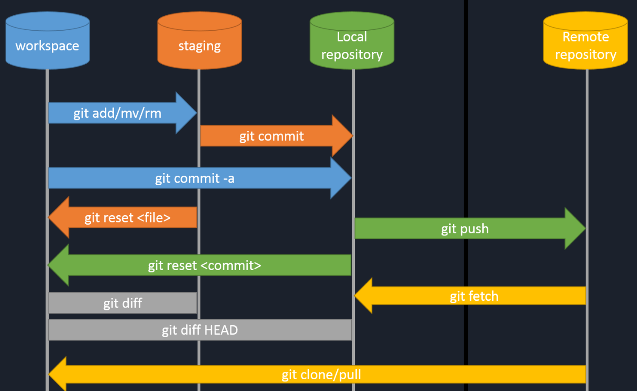
\includegraphics[width=\textwidth]{DeroulementProtocoleGit}
\end{figure}

\section{Travailler avec des branches}
\paragraph{}Les branches font parties du cœur même de Git et constituent un de ses principaux atouts. C’est un moyen de travailler en parallèle sur d’autres fonctionnalités. C’est comme si vous aviez quelque part une "copie" du code source du projet qui vous permettrait de tester vos idées les plus folles et de vérifier si elles fonctionnent avant de les intégrer au véritable code source de votre projet.

Dans Git, toutes les modifications que vous faites au fil du temps sont par défaut considérées comme appartenant à la branche principale appelée "master" :

\begin{figure}[h]
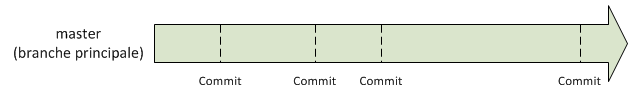
\includegraphics[width=\textwidth]{Branch1}
\end{figure}

\paragraph{}Supposons que vous ayez une idée pour améliorer la gestion des erreurs dans votre programme mais que vous ne soyez pas sûrs qu’elle va fonctionner : vous voulez faire des tests, ça va vous prendre du temps, donc vous ne voulez pas que votre projet incorpore ces changements dans l’immédiat.

Il suffit de créer une branche, que vous nommerez par exemple "idee\_gestion\_erreurs", dans laquelle vous allez pouvoir travailler en parallèle :

\begin{figure}[h]
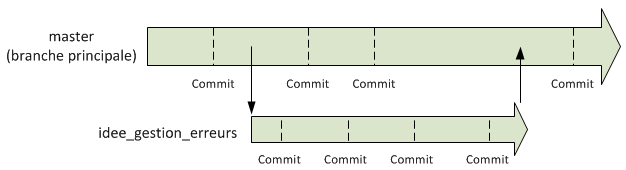
\includegraphics[width=\textwidth]{Branch2}
\end{figure}

\paragraph{}À un moment donné, nous avons décidés de créer une nouvelle branche. Nous avons pu y faire des commits, mais cela ne nous a pas empêché de continuer à travailler sur la branche principale et d’y faire des commits aussi.

Git gère tous ces problèmes pour vous. Au lieu de créer une copie des fichiers, il créé juste une branche "virtuelle" dans laquelle il retient vos changements en parallèle. Lorsque vous décidez de fusionner une branche (et donc de ramener vos changements dans "master" pour les valider), Git vérifie si vos modifications n’entrent pas en conflit avec des commits effectués en parallèle. S’il y a des conflits, il essaie de les résoudre tout seul ou vous avertit s’il a besoin de votre avis (c’est le cas si deux personnes ont modifiées la même ligne d’un même fichier par exemple).

Ce concept de branches très légères qui ne nécessitent pas de copier les fichiers est d’une grande puissance. Cela vous encourage à créer des branches tout le temps, pour toutes les modifications qui pourraient prendre du temps avant d’être terminées.

Vous pouvez même créer une sous-branche à partir d’une branche !


\subsection{Les branches locales}
\paragraph{}Tout le monde commence avec une seule branche "master" : c’est la branche principale. Jusqu’ici, vous avez donc travaillé dans la branche "master", sur le "vrai" code source de votre projet.

Pour voir toutes vos branches, tapez ceci :
\begin{lstlisting}
$ git branch
\end{lstlisting}

\paragraph{}La branche sur laquelle vous vous trouvez est indiquée par une étoile *.

\subsubsection{Pourquoi créer une branche et quand la créer ?}
\paragraph{}Lorsque vous vous apprêtez à faire des modifications sur le code source, posez-vous les questions suivantes :
\begin{itemize}
\item Ma modification sera-t-elle rapide ?
\item Ma modification est-elle simple ?
\item Ma modification nécessite-t-elle un seul commit ?
\item Est-ce que je vois précisément comment faire ma modification d’un seul coup ?
\end{itemize}

\paragraph{}Si la réponse à l’une de ces questions est "non", vous devriez probablement créer une branche. Créer une branche est très simple, très rapide et très efficace. Il ne faut donc pas s’en priver.

\subsubsection{Créer une branche et changer de branche}
\paragraph{}Imaginons que vous vouliez créer un tutoriel Web sur Git et l'insérer sur votre site internet. Vous n’êtes pas sûrs du temps que cela va prendre, ce n’est pas un changement simple qui consiste à modifier deux-trois liens et vous risquez de faire plusieurs commits. Bref, il faut créer une branche pour cela.
\begin{lstlisting}
$ git branch Tuto_Git
\end{lstlisting}

\paragraph{}Cette commande va créer une branche du nom de \emph{Tuto\_Git}, il est à noter que cette branche est locale (vous seul y avez accès), il est aussi possible de la partager sur le dépôt distant.

Vous devriez maintenant voir votre nouvelle branche en faisant un \emph{git branch}, mais vous n'êtes pas encore sur votre nouvelle branche. Pour changer de branche il vous faudra taper la commande suivante:
\begin{lstlisting}
$ git checkout Tuto_Git
\end{lstlisting}

\paragraph{}Qu’est-ce qui se passe lorsque l’on change de branche ? En fait, vous ne changez pas de dossier sur votre disque dur, mais Git change vos fichiers pour qu’il reflète l’état de la branche dans laquelle vous vous rendez. Imaginez que les branches dans Git sont comme des dossiers virtuels : vous "sautez" de l’un à l’autre avec la commande \emph{git checkout}. Vous restez dans le même dossier, mais Git modifie les fichiers qui ont changés entre la branche où vous étiez et celle où vous allez.

Sachant que si vous avez fait des modifications non-enregistrées, Git va être gentil et ne va pas écrire par dessus lors d'un checkout.

\subsubsection{Fusionner les changements}
\paragraph{}Lorsque vous avez fini de travailler sur une branche et que celle-ci est concluante, il faut "fusionner" cette branche vers "master". Pour cela commencer par vous rendre sur votre branche "master", puis exécutez la commande suivante:
\begin{lstlisting}
$ git merge Tuto_Git
\end{lstlisting}

\paragraph{}Cette commande aura pour effet de fusionner les changements
effectués dans votre branche "Tuto\_Git" dans votre branche "master", mais pas
de supprimer cette branche qui ne sert plus a rien. Pour supprimer vos
anciennes branches il vous suffira d'exécuter la commande suivante:
\begin{lstlisting}
$ git branch -d Tuto_Git
\end{lstlisting}

\paragraph{}Git vérifie que votre travail dans la branche "Tuto\_Git" a bien été fusionné dans "master". Sinon, il vous en avertit et vous interdit de supprimer la branche (vous risqueriez sinon de perdre tout votre travail dans cette branche !).

Si vous souhaitez supprimer une branche sans en sauvegarder les changements vous pouvez utiliser cette commande à la place:
\begin{lstlisting}
$ git branch -D Tuto_Git
\end{lstlisting}

\subsection{Les branches partagées}
\paragraph{}Il est possible de travailler à plusieurs sur une même branche. En fait, c’est déjà ce que vous faisiez en travaillant sur la branche "master".

Pour voir toutes les branches partagées du dépôt distant il faut utiliser la commande suivante:
\begin{lstlisting}
$ git branch -r
\end{lstlisting}

\paragraph{} Si le serveur possède une autre branche, par exemple
"origin/brancheserveur", et que vous souhaitez travailler dessus, il suffit
d'utiliser la commande suivante:

\begin{lstlisting}
$ git checkout brancheserveur
\end{lstlisting}

\paragraph{}Lorsque vous ferez un pull depuis la branche "brancheserveur", les changements seront fusionnés dans votre "brancheserveur" local. Il est donc important de savoir dans quelle branche vous vous trouvez avant de faire un pull. Un pull depuis la branche "master" met à jour votre branche "master" locale en fonction de ce qui a changé sur le serveur, et il en va de même pour n’importe quelle autre branche.

\paragraph{} Voyons maintenant comment créer et supprimer vos propres branches
partagées. Si vous avez créé une branche localement, et que vous voulez "push"
les modifications sur le serveur il vous suffit de faire:

\begin{lstlisting}
$ git push --set-upstream origin ma_nouvelle_branche
\end{lstlisting}

\paragraph{} Les options de "git push" signifient que votre nouvelle branche
sera liée à votre dépôt distant, représenté par le mot "origin". Une fois cette
liaison faite, les commandes "git push" et "git pull" fonctionneront
automatiquement sans options, pourvu que vous soyez sur la bonne branche.

\paragraph{} Enfin voyons comment supprimer une branche partagée du serveur,
pour cela il suffit d'utiliser la commande suivante:

\begin{lstlisting}
$ git push --delete origin nom_branche_a_supprimer
\end{lstlisting}

\paragraph{} À noter que cette commande supprime uniquement la branche sur le
serveur. Il vous faudra tout de même supprimer votre branche locale comme vu à
la section précédente.

\newpage
\part{Conclusion}
\paragraph{}Maintenant vous devriez avoir une idée de ce qu'est Git et de comment il va pouvoir vous être utile !

Vous devriez être capable de connaître les opérations basiques : créer ou cloner un dépôt, effectuer un commit ou des modifications et être capable de visualiser les modifications de chaque version dans un même projet.
Nous avons enfin couvert la création de branches, le changement de branche et la fusion de branches locales.
Vous devriez aussi être en mesure de partager vos branches sur un serveur et de travailler à plusieurs sur des branches partagées.

Le club Nix reste à votre disposition si vous avez besoin d'aide ou désirez poser une question.

\section*{Bibliographie}

\begin{itemize}
	\item LE site de l'origine avec les documentations originelles: \url{http://git-scm.com}
\end{itemize}

\paragraph{}Et de la lecture en anglais
\paragraph{}
Si nous n'avons pas été clair, deux résumés :
\begin{itemize}
	\item \url{http://rogerdudler.github.io/git-guide/}
	\item \url{https://www.atlassian.com/git/}
\end{itemize}


\paragraph{}
Un guide pour écrire de bons messages de commit :

\url{https://juffalow.com/other/write-good-git-commit-message}



\paragraph{}Sachant que vous pouvez TOUT trouver sur Git, du bon comme du mauvais, amusez vous bien \textbackslash o/

%TODO
% Explain why `git init --bare' if on own server
\end{document}
% vim: spell : spelllang=fr
